\chapter{Appendix A}

 \subsection{Wave-data check}
 
Estimation of fetch-limited Waves; Method of Verhagen and Young: \\
$ \tilde{H}=\tilde{H}_{\infty}[tanh(k_1 \tilde{F}^{m_1})]^p $ with $ \tilde{F}= \frac{g F}{U_{10}^2} $ and $H_{m0} = \frac{\tilde{H} U_{10}^2}{g} $ \\
The input:
\begin{itemize}
\item $\tilde{H}_{\infty}= 0.24 $
\item $k_1= 4.41*10^{-4} $
\item $ m_1= 0.79 $
\item $p= 0.572 $
\item $F= 1000 km $
\item $U_{10}= 20 \frac{m}{s} $
\end{itemize}
 and the results:
 \begin{itemize}
 \item $\tilde{F}=25000 $
 \item $\tilde{H}= 0.22 $
 \item $H_{m0}= 8.8 m $
 \end{itemize}
 8.8 m is the maximum possible wave hight according to the fetch length and the Young/Verhagen method of dimensionless fetch.
 \subsection{Wave and Wind informations}
\begin{figure}[H]
\center
\fbox{
 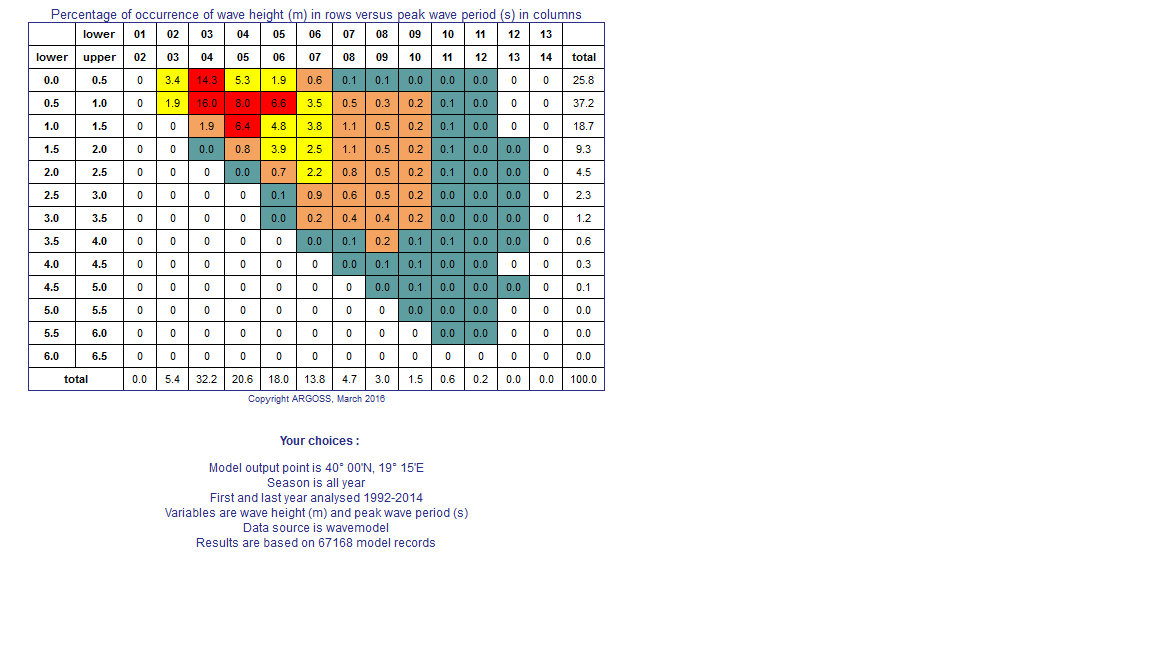
\includegraphics[width=\textwidth]{images/wave_pperiod_allyear.png} 
}
\caption[Distribution of peak-period over wave hight]{Distribution of peak-period over wave hight}
 %\label{Distribution_pperiod}
\end{figure}
% 
% 
\begin{figure}[H]
\center
\fbox{
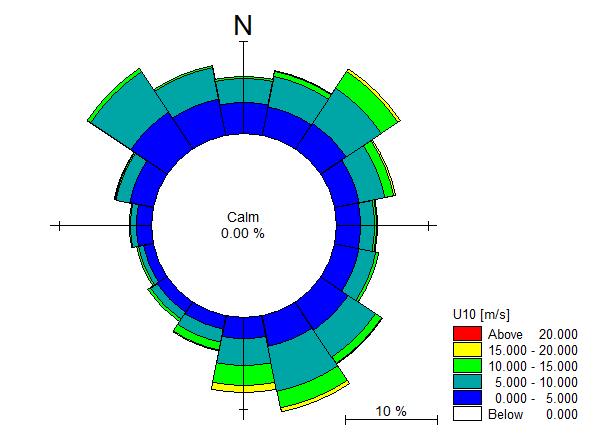
\includegraphics[width=\textwidth]{images/Rose_plot_u10.png} 
}
\caption{Rose-diagram with the distribution of the wind}
 %\label{Windrose}
\end{figure}
% 
% 
\begin{figure}[H]
\center
\fbox{
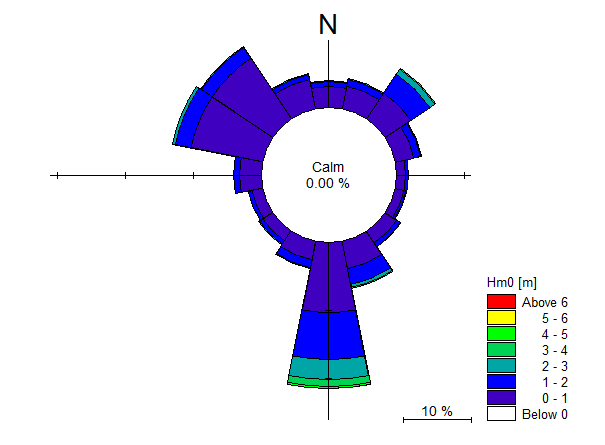
\includegraphics[width=\textwidth]{images/Rose_plot_Hoverall.png} 
}
\caption{Rose-diagram with the distribution of the waves}
% %\label{wavedata_angle}
\end{figure}

\subsection{Design of Armour Layer Cubes}
\begin{center}
\begin{table}[!htb]
\begin{tabu}{X[2l] X[2l] X[2c]}
\toprule[2pt]
\textbf{Parameter} & \textbf{Short Description} &\textbf{Value} \\
\\
\midrule
$H_{sig}$  & Significant wave hight & 5.6\\
\\
$T_p$ & Peak period & 11 s\\
\\
$T_m$ & Mean wave period & 8.8 s\\
\\
tr & Duration of a storm & -9 hrs \\
\\
Nod & Number of displaced armour units & 0.5\\
\\
$\rho _s$ & Mean density of stone material & 2400 $ \frac{kg}{m³} $ \\
\\
$\rho _w$ & Mean density of water & 1025  $ \frac{kg}{m³} $\\
\\
$\Delta$ & Relative buoyant density of material & 1.34\\
\\
S & Wave steepness for mean wave period & 2\\
\\
Dn & Nominal diameter of armour units & 2.09 m\\
\midrule
\multicolumn{1}{c}{Results}\\ \cmidrule{1-3}
%\midrule
Dn & Nominal diameter of armour units & 2.14 m\\
\\
M & Mass of stone & 23638 kg\\
\bottomrule[2pt]
\end{tabu}
\caption{Design Armour Layer}
\label{tab:design_armour}
\end{table}
\end{center}

\begin{figure}[H]
\center
\fbox{
\includegraphics[width=\textwidth]{images/Design_Armour1.png} 
}
\caption{Cress Design Equation and Explanation}
% %\label{Design_Armour1}
\end{figure}

Whatever XX
